\documentclass{article}
\usepackage{amsmath}
\usepackage{tikz}
\usetikzlibrary{arrows.meta}

\begin{document}

\begin{figure}[h]
    \centering
    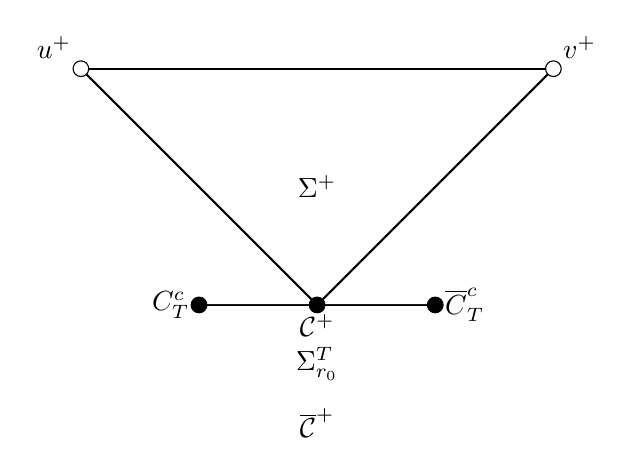
\begin{tikzpicture}[scale=1.5]
        % Define coordinates
        \coordinate (A) at (-2, 2);
        \coordinate (B) at (2, 2);
        \coordinate (C) at (0, 0);
        \coordinate (D) at (-1, 0);
        \coordinate (E) at (1, 0);
        
        % Draw the main lines
        \draw[thick] (A) -- (B);
        \draw[thick] (A) -- (C);
        \draw[thick] (B) -- (C);
        \draw[thick] (D) -- (C);
        \draw[thick] (E) -- (C);
        
        % Draw the dashed line
        \draw[dashed] (A) -- (B);
        
        % Draw the shaded area
        \fill[gray!30] (D) -- (C) -- (E) -- cycle;
        
        % Label points
        \node at (A) [circle, draw, fill=white, inner sep=2pt] {};
        \node at (B) [circle, draw, fill=white, inner sep=2pt] {};
        \node at (C) [circle, draw, fill=black, inner sep=2pt] {};
        \node at (D) [circle, draw, fill=black, inner sep=2pt] {};
        \node at (E) [circle, draw, fill=black, inner sep=2pt] {};
        
        % Add labels
        \node at (A) [above left] {$u^+$};
        \node at (B) [above right] {$v^+$};
        \node at (C) [below] {$\mathcal{C}^+$};
        \node at (D) [left] {$C_T^c$};
        \node at (E) [right] {$\overline{C}_T^c$};
        \node at (0, 1) {$\Sigma^{+}$};
        \node at (0, -0.5) {$\Sigma_{r_0}^T$};
        \node at (0, -1) {$\overline{\mathcal{C}}^+$};
        
    \end{tikzpicture}
    \caption{Spacetime region on which we solve the wave equation up to the cosmological horizons. We solve a sequence of finite problems, i.e., we consider a solution $\psi_T$ with prescribed data on $\Sigma_{r_0}^T \cup C_T^c \cup \overline{C}_T^c$, and then show that the limit $\lim_{T \to \infty} \psi_T$ exists in a suitable energy space.}
    \label{fig:spacetime_region}
\end{figure}

\end{document}